
\lhead[\chaptername~\thechapter]{\rightmark}

\rhead[\leftmark]{}

\lfoot[\thepage]{}

\cfoot{}

\rfoot[]{\thepage}

\chapter{Introduction}\label{introduction}

\section{Overview}

The influence of wearable technology on our lives is gradually getting stronger and they are becoming part of our lives. 
Image classification and image retrieval systems are widely used on smart phones or other wearable devices.
As the personal usage of these systems are becoming more and more popular, the need for faster and more efficient architectures is evident. 

Image classification and image retrieval systems are commonly implemented with multi-purpose functionality to satisfy a wide range of users. 
In image classification, deep learning models are trained to recognize hundreds of class categories and the models become large in memory and computationally expensive as a consequence.
In the same manner, search algorithms for image retrieval systems browse the entire area of the search space with billions of images.
However, people's surroundings, their occupation, hobbies and interests and various other things affect their usage of these systems.
Each user's needs to use these systems are different from each other.
A user may want to recognize a certain breed of an animal 
whereas another user may require to distinguish between kitchen utensils.
Moreover, some users may never see a physics laboratory, but some other users might be working in one.
Because the personal usage of these systems is spreading widely, 
usage requirements of the users should be used to make these systems more efficient.

We propose a novel solution for both image classification and image retrieval tasks 
that makes use of user requirements to make the systems more efficient and faster while maintaining the accuracy.
Solutions for each task will be introduced in their corresponding sections.



\section{Image Classification}
\label{sec:intro}

In the recent years, convolutional neural networks (CNNs) have become widely used in many areas including personal use. 
Individual uses are supported by service providers who make use of the high-performance computers. 
Service providers train and deploy deep neural network models and 
users download and use the trained models for their specific purposes.
Generally, wearable devices have limited resources such as computational power or restricted memory size. 
Despite this limitation, deep learning models commonly require high computational power and memory usage.

In many cases, there is a conflict of interest between service providers and the users.
On the one hand, service providers often train a very deep model with high-performance computers to achieve accurate and multi-purpose recognition. 
On the other hand, end-users may have to run the models with a more limited computational resources, e.g., smartphones and wearable devices. 
Moreover, the users do not always require the whole multi-purpose recognition capabilities. 
For instance, they may only need to distinguish a couple of objects they interact with everyday, out of the 1000 diverse classes that can be recognized by training from ImageNet~\cite{deng2009imagenet}.

One straightforward idea to mitigate this gap between service providers and users is 
to compress the model based on each individual user's requirements and 
distribute the personally compressed models to the corresponding users. 
However, it is infeasible to compress the models for every combination of classes and satisfy every single user. 

A solution to above mentioned method would be to ask the users to compress models based on their needs to make it executable with their computational resources and memories and also simple enough for their purposes. 
However, much relevant work requires re-training of the models at user side, 
such as model distillation and pruning, 
which is not always possible given the limited computational power users have.

\begin{figure}
    \centering
    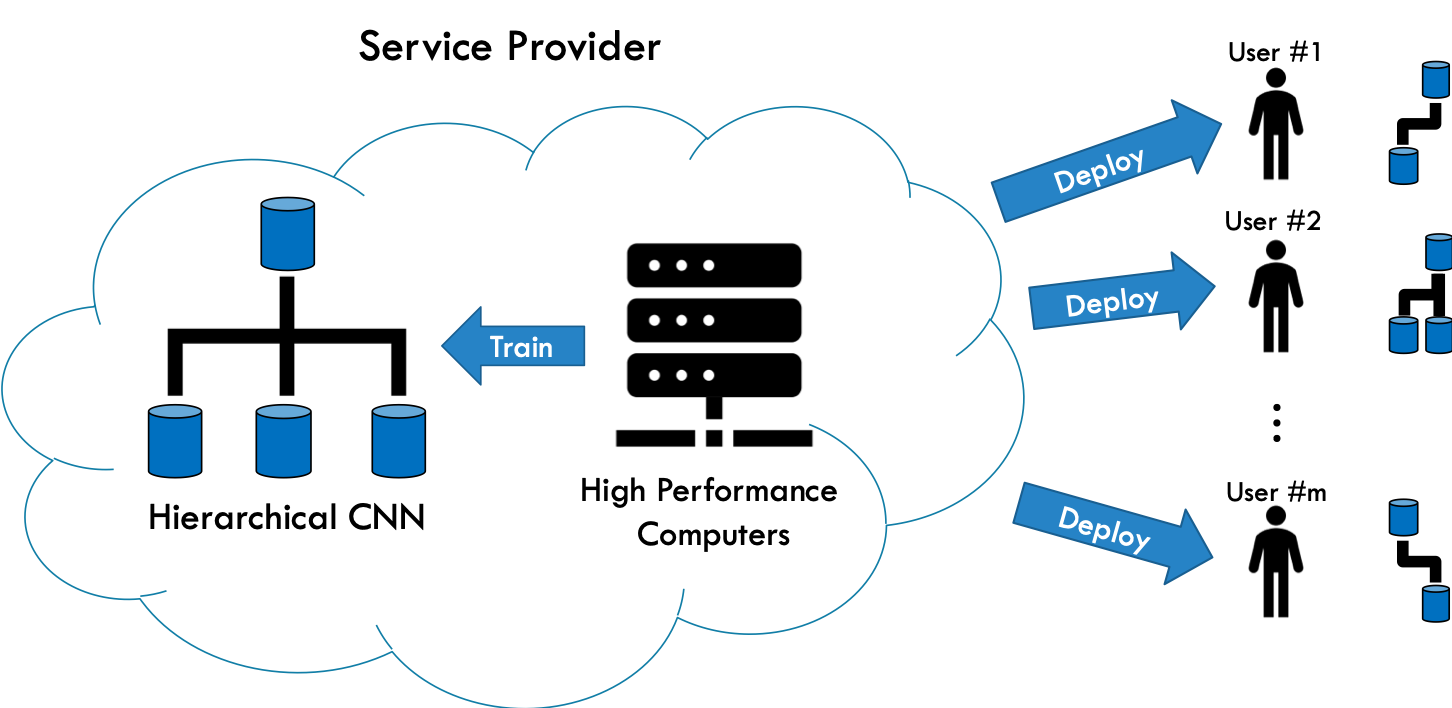
\includegraphics[width=.7\textwidth]{images/ArchitectureOverview(ver2).png}
    \caption{Overview of our scenario-based solution}
    \label{fig:overview}
\end{figure}

We propose a new training strategy that 
allows the users to use a limited part of the trained model based on the classes they encounter in their surroundings. 
The key idea is that the users with different requirements make use of a partially executable model that is trained on service provider side with high computational resources.
This adaptive use allows users to obtain personal simpler models that can run on their devices 
that are limited in memory and computational power without the necessity of re-training the obtained model. 

More specifically, our solution works as in figure \ref{fig:overview}. 
Service providers train a hierarchical
general-purpose network with recognition capabilities of all the possible classes 
that is separable to sub-parts that each recognizes a subset of the classes. 
End-users download and use the part of the network that includes their required subset of the classes.
In this way, each user obtains a smaller model that is tailored for their individual needs.

Additionally, if the users encounter a class that is not in their model, 
the proposed system has the functionality to detect the irregular class and 
downloads extra parts from the full model on the service provider side. 
Thus, the users have access to all the functionality of the complete model if they require.

To evaluate our solution in a scenario-based fashion, 
in our experiments we assume that 
each user encounters a random subset of classes much more likely than 
the rest of the classes due to the limitation of their surroundings. 
Therefore, we tested our approach on generated realistic test users with a biased probability of encountering a subset of classes.

Our hierarchical CNN model is based on a backbone neural network architecture, namely we used VGG16~\cite{simonyan2014very} and MobileNet~\cite{howard2017mobilenets}. 
We compared our solution, hierarchical tree-shaped CNN with \textit{N} branches, with baseline methods for both accuracy and average storage cost for each user. 
We considered two baseline methods, the first one is the backbone CNN that recognize all possible classes 
whereas the second one is \textit{N} smaller models each recognizing a subset of classes.
The latter method differs from our method in the sense that the models do not share any parameters. 
Lastly, we worked with CIFAR-10 dataset to compare our method with the baseline methods.
Experimental results showed that memory usage per user can be nearly halved with similar accuracy.

\section{Image Retrieval}

With the advent of internet, everybody has access to enormous amount of digital image data. 
Searching through this big data has become a very important task. 
Image retrieval is widely used in many applications 
in which there is an image search functionality. 
In this work, we mainly focus on content-based image retrieval (CBIR)
where the content of the image itself is used to search
as opposed to using meta-data or descriptive data of an image.

In image retrieval task, the images are represented with a vector.
Then the task is to find the closest vector to a query vector in a predefined search space. 
Because brute-force searching takes a lot of time, many methods use Approximate Nearest Neighbor (ANN) search for efficiency. 
In ANN algorithms, the search space is divided into sub-spaces. 
When a query vector comes, firstly a few sub-spaces are selected with a high likelihood of containing the true result, 
then only the vectors in those sub-spaces are searched.
Therefore, the search speed is faster with a high probability of finding the true result.

Our idea is to reduce the search space according to the user requirements to speed up the search. 
Query vectors are usually assumed to have the same distribution with the searched database. 
However, query images of each user are restricted to user's interests, occupations and mostly their surroundings.
For example in a similar scene image search, a pilot and a police officer would have completely different query images.
Provided that most of the query images are coming from only a part of the search space, the ANN search can be done in that limited space. 
By exploiting the query distribution of each user, it is possible to personalize their search to make it faster.

In our method, we use the classification labels of the images to learn the user requirements. 
We use places365~\cite{zhou2017places} dataset images to construct the search database and the classification label information to realize user requirements.
Supposing that the most query images of the users are classified into a few number of class labels, we can reduce the search space by eliminating sub-spaces not containing those labels.
After limiting the area of the search, ANN search can be performed in the remaining sub-spaces.
Results of our experiments with artificial data revealed that the search becomes faster with a small or no decrease in accuracy. 
However, experimental results with real-life data suggested that more improvement is needed to speed up the image search for a real-life example.


\section{Thesis Outline}

The rest of the thesis is organized as follows. 
In chapter \ref{related}, related work of image classification and image retrieval part will be explained in their respective sections. In chapter \ref{method}, section \ref{sec:HierCNN} will introduce our proposed method on Image classification. 
Details of constructing the hierarchy, obtaining CNN model from the hierarchy, generating realistic users and the baseline of our work will be given. 
Following section \ref{sec:FasterANN} will talk about the method of obtaining vector representation of images, reducing the search space with our proposed method and the baseline in detail.
In Chapter \ref{experiments}, experiments will be shared for each task and the results will be discussed and analyzed in chapter \ref{discussion}. Finally, in chapter \ref{conclusion}, future work will be mentioned along with the conclusive remarks.

